%%%%%%%%%%%%%%%%%%%%%%%%%%%%%%%%%%%%%%
% Numerical Linear Algebra class 2022 
% Solutions to Sheet 8
%%%%%%%%%%%%%%%%%%%%%%%%%%%%%%%%%%%%%%

\begin{SolutionSheet}[\ref{sheet8}]

  \begin{Solution}[{\cite[P-5.1 b]{Saad00}}]
  	\hfill\\
  	Part (a):
  	
    Hint 1:
    \begin{gather*}
      \scal(\mata\vd^{(k+1)},\vd^{(k+1)})
      =\scal(\mata\vd^{(k)},\vd^{(k)})
      -\frac{\scal(\vr^{(k)},\ve_i)^2}{a_{ii}}
    \end{gather*}

    Hint 2:
    \begin{gather*}
      \abs{\ve_i^T \vr^{(k)}} \geq n^{-\nfrac12}\norm{\vr^{(k)}}_2
    \end{gather*}

    With the help of hint 1 and 2 we get
    \begin{align*}
      \norm{\vd^{(k+1)}}_{\mata}^2
      = \scal(\mata\vd^{(k+1)},\vd^{(k+1)})
      &\stackrel{\text{Hint 1}}{=}
        \scal(\mata\vd^{(k)},\vd^{(k)})
        - \frac{\scal(\vr^{(k)},\ve_i)^2}{a_{ii}}
      \\
      &=
        \left( 1 - \frac{\scal(\vr^{(k)},\ve_i)^2}{a_{ii}}
              \frac1{\scal(\mata\vd^{(k)},\vd^{(k)})} \right)
        \norm{\vd^{(k)}}_{\mata}^2
      \\
      &\stackrel{\text{Hint 2}}{\leq}
        \left( 1 - \frac{1}{n a_{ii}}
              \frac{\norm{\vr^{(k)}}_2^2}{\scal(\mata\vd^{(k)},\vd^{(k)})} \right)
        \norm{\vd^{(k)}}_{\mata}^2
    \end{align*}
    The result follows by the following two estimates of Rayleigh quotients:
    \begin{gather*}
      a_{ii} = \scal(\mata\ve_i,\ve_i) = \frac{\scal(\mata\ve_i,\ve_i)}{\scal(\ve_i,\ve_i)}
      \le \lambda_{\max},
    \end{gather*}
    and
    \begin{gather*}
      \frac{\scal(\mata\vd^{(k)},\vd^{(k)})}{\norm{\vr^{(k)}}^2}
      = \frac{\scal(\vr^{(k)},\mata^{-1}\vr^{(k)})}{\norm{\vr^{(k)}}^2}
      \le \lambda_{\max}(\mata^{-1})
      = \frac1{\lambda_{\min}}.
    \end{gather*}
    
    Part (b): For $n > 1$, $1-\frac1{n\cond(\mata)} < 1$, and thus
    \[\norm{\vd^{(k+1)}}_\mata \leq \left(1-\frac1{n\cond(\mata)}\right)^{\frac{k+1}{2}}
    \norm{\vd^{(0)}}_\mata \rightarrow 0 \text{ for } n\rightarrow \infty.\]
    That shows that $x^{(k)}$ converges to the solution $x = \mata^{-1}\vb$.
    

    Final remarks:\\
    1. Since $\ve_i\in K=L$, it holds the Galerkin-orthogonality
    \begin{align*}
      \scal(\vr^{(k)}-\alpha\mata \ve_i,\ve_i) = 0,
    \end{align*}
    where according to Example 2.3.10
    \begin{gather*}
      \alpha = \frac{\scal(\vr^{(k)},\ve_i)}{\scal(\mata\ve_i,\ve_i)}
      = \frac{\scal(\vr^{(k)},\ve_i)}{a_{ii}}
      .
    \end{gather*}
    This would have been used to show hint 1.

    2. To show hint 2, notice that by the choice of $i$ as maximal
    value of the residual vector
    \begin{align*}
      \norm{\vr^{(k)}}_2
      \leq \sqrt{n} \norm{\vr^{(k)}}_{\infty}
      = \sqrt{n} \abs{\ve_i^T\vr^{(k)}}
    \end{align*}

  \end{Solution}

  \begin{Solution}
  	Part (a): 
  	\begin{equation*}
  	\vp = \mata \vr - \frac{\scal(\mata\vr,\vr)_{\mata}}{\scal(\vr,\vr)_{\mata}} \vr.
  	\end{equation*}
  	Then $\scal(\mata\vr,\vp)=\scal(\vr,\vp)_{\mata}}=0$.
  	
  	Part(b): As defined in Definition 3.3.3, we choose $\vv\in K=L$, i.e. $\vv$ is a linear combination of $\vp$ and $\vr$.
  	From the second condition $\vr^{(k)} - \mata\vv \perp L$, we can deduce the coefficients for v:
  	\begin{equation*}
  	\vr^{(k)} - \mata\vv \perp L \Rightarrow \scal(\vr-\mata\vv,\vr) = 0,\scal(\vr-\mata\vv,\vp)=0.
  	\end{equation*}
  	
  	Let $\vv = \alpha \vr + \beta\vp$.
  	\begin{align*}
  		\scal(\vr-\mata\vv,\vr) &= 0\\
  		\Leftrightarrow \scal(\vr,\vr) - \scal(\alpha\mata\vr + \beta\mata\vp,\vr) &= 0\\
  		\Leftrightarrow \scal(\vr,\vr) - \alpha\scal(\mata\vr,\vr) - \beta\scal(\mata\vp,\vr) &= 0\\
  		\Leftrightarrow \scal(\vr,\vr) - \alpha\scal(\mata\vr,\vr) - \beta\scal(\vp,\mata\vr) &= 0\\
  		\Leftrightarrow \scal(\vr,\vr) - \alpha\scal(\mata\vr,\vr) &= 0\\
  		\Leftrightarrow \alpha &= \frac{\scal(\vr,\vr)}{\scal(\mata\vr,\vr)}
  	\end{align*}
  	
  	\begin{align*}
  		\scal(\vr-\mata\vv,\vp) &=0\\
  		\Leftrightarrow \scal(\vr,\vp) - \scal(\alpha\mata\vr + \beta\mata\vp,\vp) &= 0\\
  		\Leftrightarrow \scal(\vr,\vp) - \alpha\scal(\mata\vr,\vp) - \beta\scal(\mata\vp,\vp) &=0\\
  		\Leftrightarrow \scal(\vr,\vp) - \beta\scal(\mata\vp,\vp) &=0\\
  		\Leftrightarrow \beta &= \frac{\scal(\vr,\vp)}{\scal(\mata\vp,\vp)}\\
  		\Leftrightarrow \beta &= \frac{\scal(\vr,\vp)}{\scal(\mata^2\vr,\vp)}.
  	\end{align*}
  	
  	In each step, first update $\vp$, then compute $\alpha$ and $\beta$ and then update $\vx$.
  	
  	
  	Part (c): The method is similar to the steepest decent method.
  	In the steepest decent method we choose $K_{\text{sd}}=L_{\text{sd}}=\spann{\vr}$ and in the method described here we choose $K = L = \spann{\vr, \mata\vr}$.
  	In each step $K_{\text{sd}}\subset K$ and $L_{\text{sd}}\subset L$. 
  	Thus, the method is not converging worse than the steepest decent method.
  	Therefore, it converges.
  \end{Solution}

  \begin{Solution}[Programming]
    C++ sample code \lstinline{./programs/steepest-decent.cc} without
    assembling the system matrix.

    Convergence rate (Definition 2.2.18 in lecture notes).  As can be
    seen in the plot, the convergence of the steepest decent method is
    sublinear.

    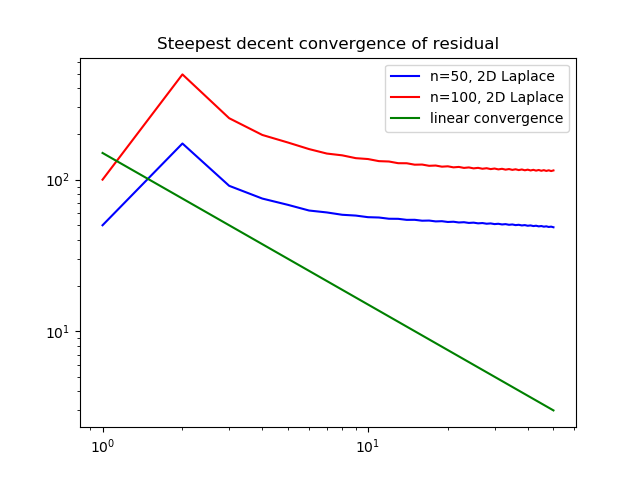
\includegraphics[width=\textwidth]{figures/laplace-steepest-decent}
  \end{Solution}

\end{SolutionSheet}


%%% Local Variables: 
%%% mode: latex
%%% TeX-master: "main"
%%% End: 
